\chapter{Appendix}
\label{appendix:equi}

\section{Density of states}

\begin{figure}[H]
	\centering
	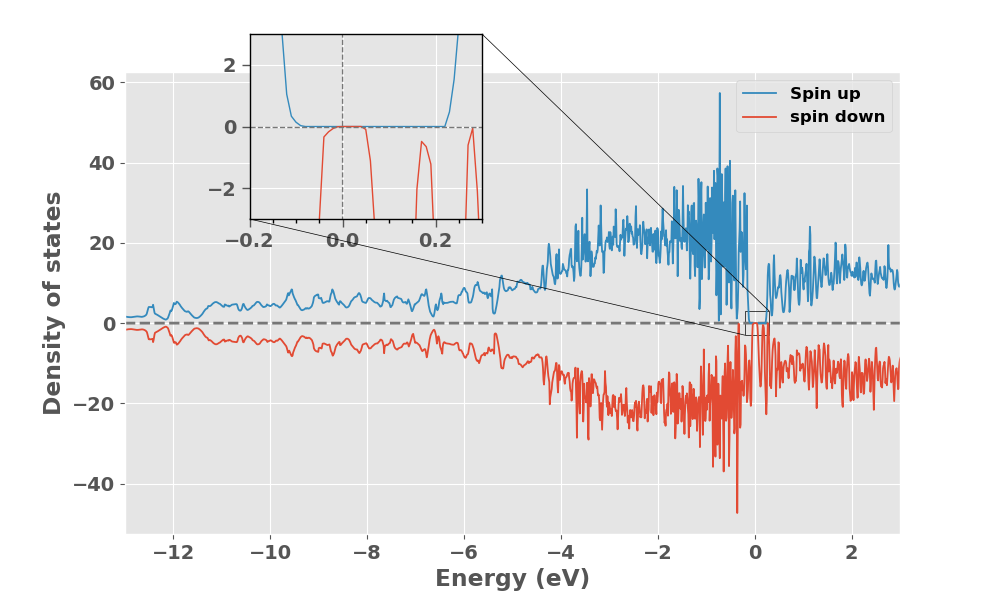
\includegraphics[width=\textwidth]{results/fesi2/E_TDOS.png}
	\caption{Density of states [states/eV] of SQS E of \ch{(CrFeMnNi)Si2}.}
\end{figure}

\begin{figure}[H]
	\centering
	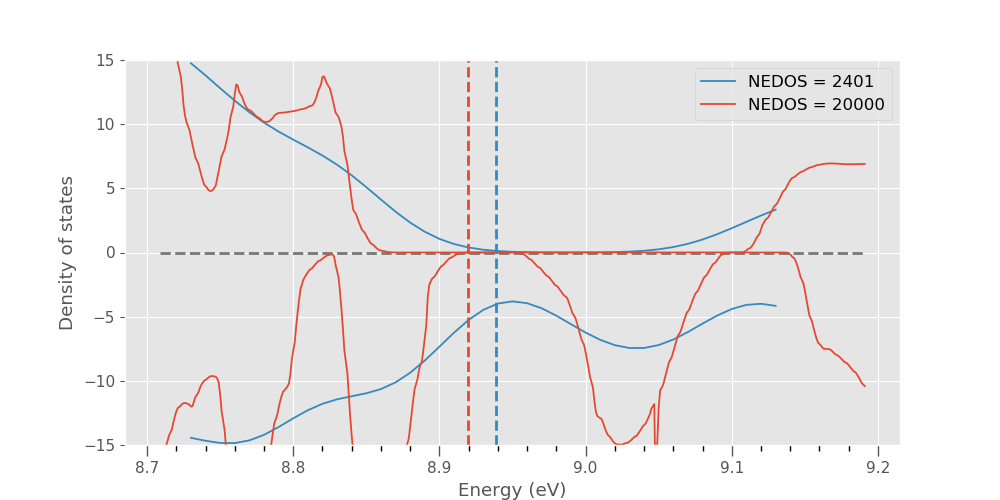
\includegraphics[width=\textwidth]{results/fesi2/C_DOS.png}
	\caption{Density of states [states/eV] of SQS C \ch{(CrFeMnNi)Si2}. NEDOS represents the number of points in the DOS calculation.}
\end{figure}

\begin{figure}[H]
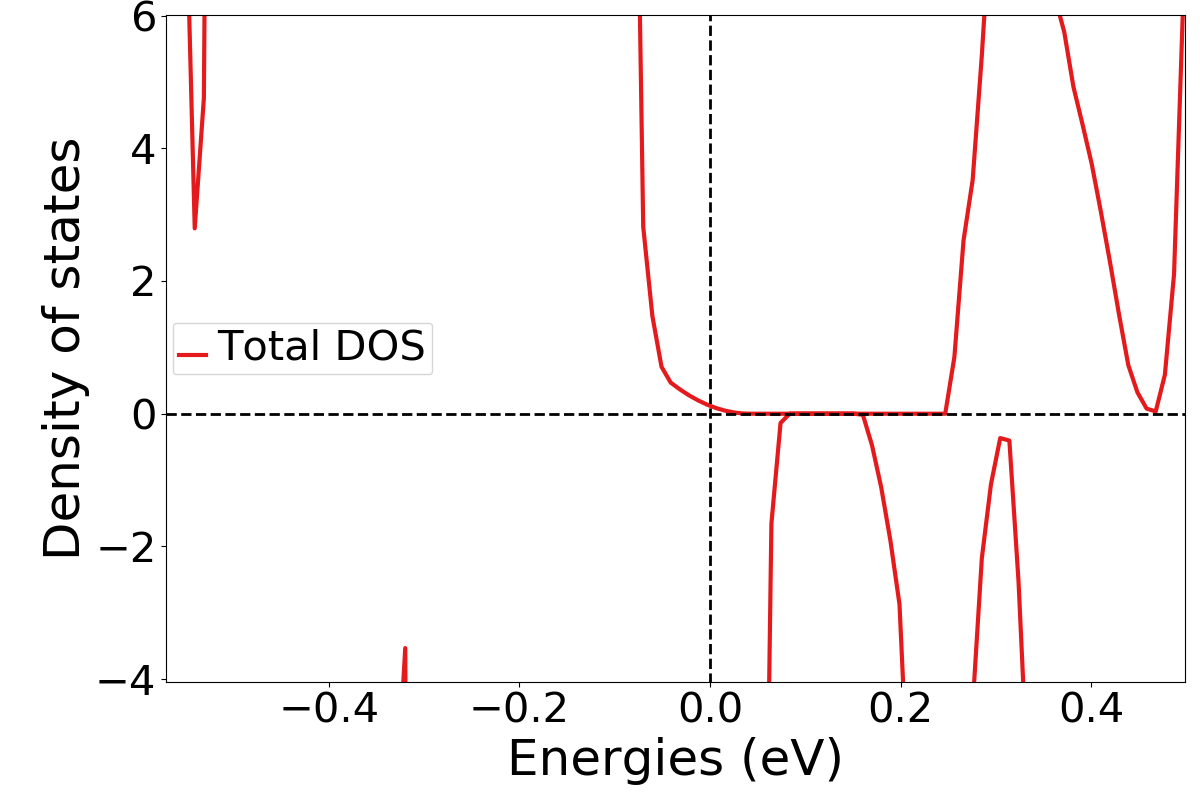
\includegraphics[width=\textwidth]{results/fesi2/permutations/mnni3_DOS_E.png}
\caption{Density of states [states/eV] of SQS C of \ch{Cr5Fe5Mn3Ni3Si32}, illustrating the small finite DOS at $E_F$ due to the impurity gap.}
\end{figure}

\section{Projected density of states}

\begin{figure}[H]
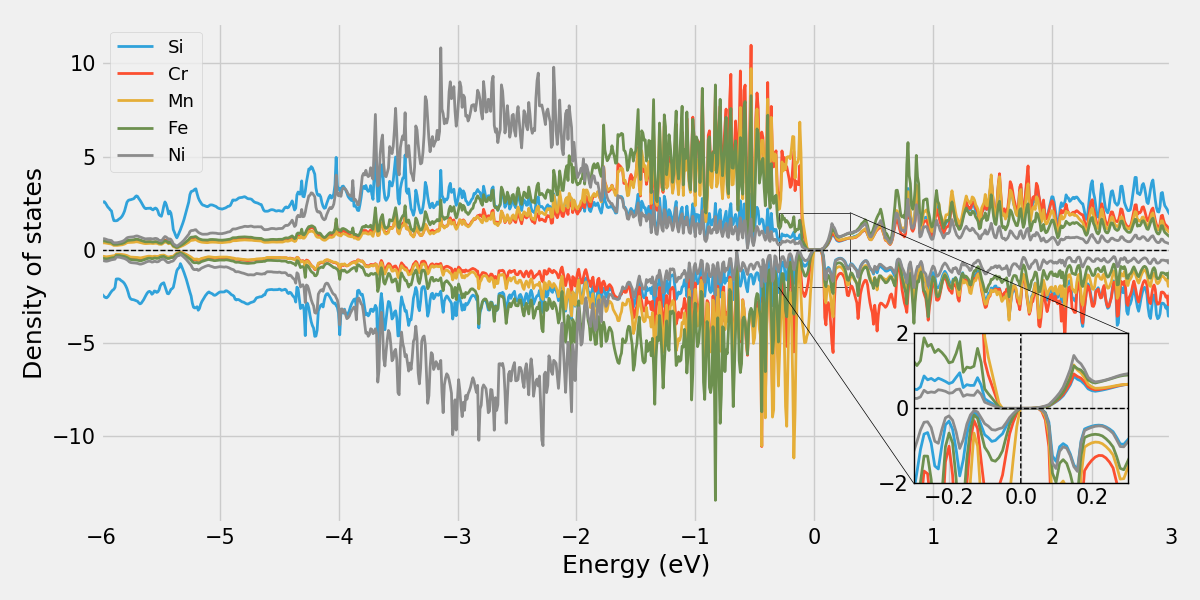
\includegraphics[width=\textwidth]{results/fesi2/A_PDOS.png}
\caption{Projected density of states [states/eV] of SQS A of \ch{(CrFeMnNi)Si2}}
\end{figure}

\begin{figure}[H]
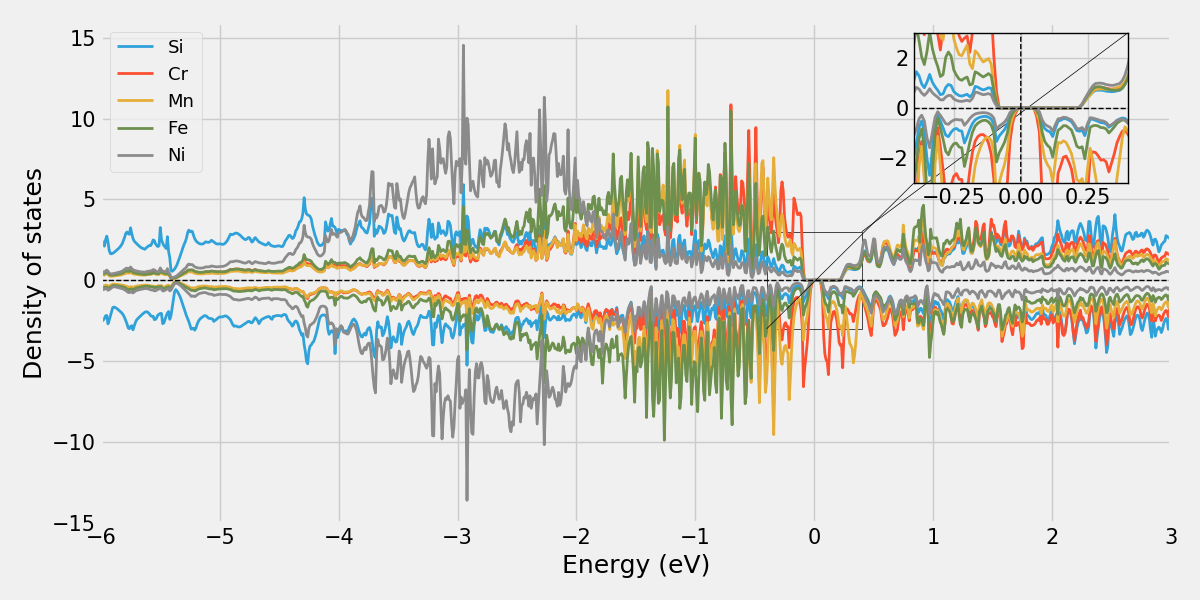
\includegraphics[width=\textwidth]{results/fesi2/B_PDOS.png}
\caption{Projected density of states [states/eV] of SQS B of \ch{(CrFeMnNi)Si2}}
\end{figure}

\begin{figure}[H]
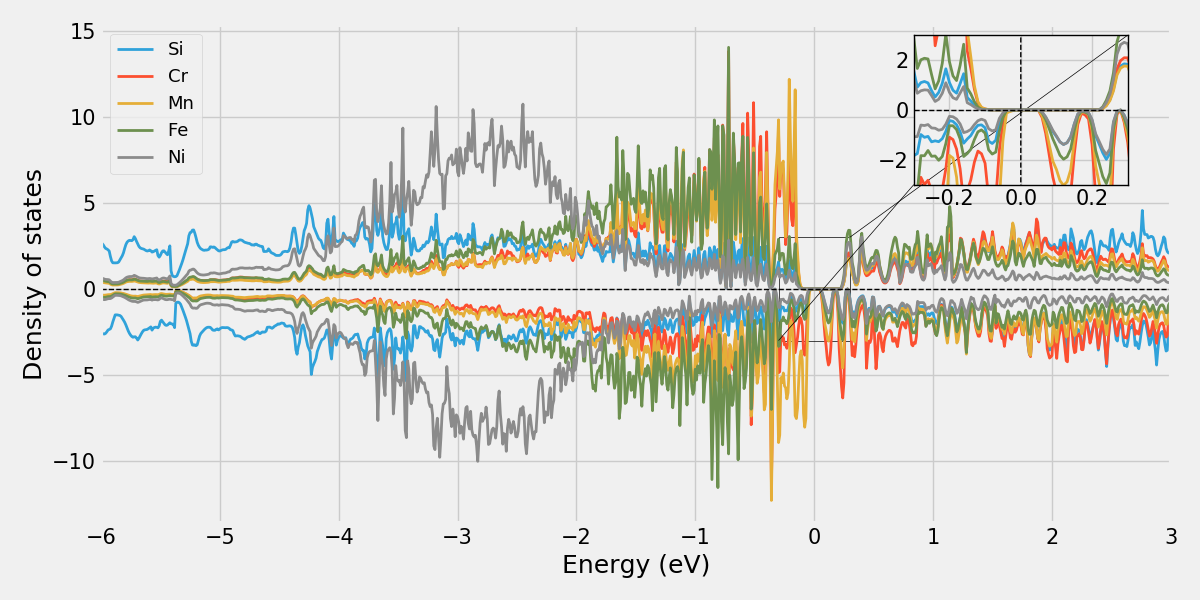
\includegraphics[width=\textwidth]{results/fesi2/E_PDOS.png}
\caption{Projected density of states [states/eV] of SQS E of \ch{(CrFeMnNi)Si2}}
\end{figure}

\section{Charge density}

\begin{figure}[H]
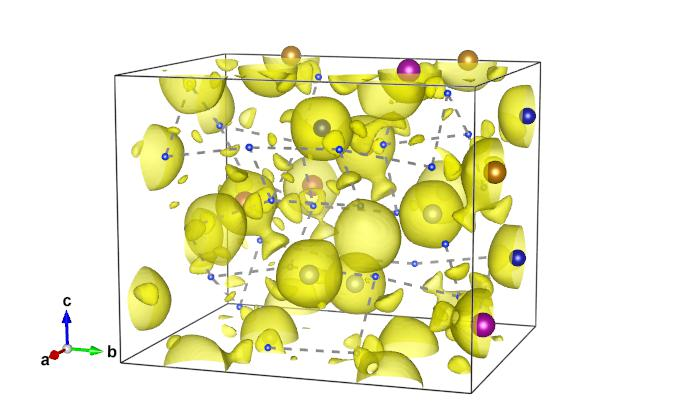
\includegraphics[width=\textwidth]{results/fesi2/C_CHGCAR.jpg}
\caption{Contour plot of the charge density of SQS C of \ch{(CrFeMnNi)Si2}.}
\end{figure}

